\section{Kondensatorn}
\marginnote{HAREC a.\ref{HAREC.a.2.2}\label{myHAREC.a.2.2}}
\index{kondensator}

\subsection{Allmänt}

Så snart det finns en elektrisk potentialskillnad --- en spänning --- mellan två
kroppar, så uppstår ett elektriskt kraftfält mellan dem. Ett sådant fält är
lagrad elektrisk energi. Kropparna måste då isoleras från varandra.

Elektrisk energi lagras mellan olika delar av en strömkrets, även om de inte är
direkt avsedda för det. Särskilt vid mycket höga frekvenser har detta stor
betydelse för utformningen av en strömkrets. Vid låga frekvenser och likström
har kretsens utformning däremot mindre inverkan. Då behövs i stället särskilda
anordningar för ta upp eller avge energi på önskade ställen i strömkretsen.

En sådan anordning kallas kondensator. Den består i princip av två band eller
plattor med anslutningsledningar samt ett isolerande skikt --- dielektrikum ---
däremellan. Kapacitansen är näst efter resistansen den vanligaste egenskapen i
en strömkrets.

\subsection{Kapacitans}
\marginnote{HAREC a.\ref{HAREC.a.2.2.1}\label{myHAREC.a.2.2.1}}
\index{kapacitans}
\index{dielektricitet}
\index{symbol!\(C\) kapacitans}
\index{symbol!\(\epsilon_0\) dielektricitetskonstanten}
\index{symbol!\(\epsilon_r\) relativa dielektricitetskonstanten}

Förmågan att lagra elektrisk energi (elektrisk laddning) kallas
\emph{kapacitans} (eng. \emph{capacitance}).
Ordet kommer från latinets capax, som betyder rymlig eller duglig.

Kapacitansen betecknas i formler med bokstaven C.

En kondensators kapacitans bestäms av ytan på kondensatorns plattor, avståndet
mellan dessa ytor, den absoluta dielektricitetskonstanten \(\epsilon_0\) och den
relativa dielektricitetskonstanten \(\epsilon_r\) som är den faktor kapacitansen
ökar med när dielektrikum är annat än vakuum.

Det isolerande materialet mellan plattorna kallas för \emph{dielektrum}
(eng. \emph{dielectrum}), och egenskaperna hos materialet påverkar kondensatorns
kapacitans.
Den egenskapen som materialet har kallas för \emph{dielektricitet}
(eng. \emph{dielectric property}) och uttrycks så som dess
\emph{dielektricitetskonstant} (eng. \emph{dielectric constant}).

Eftersom dielektriciteten ökar relativt den hos vakuum så använder man
dielektricitetskonstanten för vakuum \(\epsilon_0\) som en skalfaktor för att
omvandla den relativa dielektricitetskonstanten \(\epsilon_r\) till den
absoluta dielektricitetskonstanten \(\epsilon\).
\[
  \epsilon = \epsilon_0\epsilon_r
\]

Den relativa dielektriska konstanten går att hitta i tabeller och varierar
med material. Dielektricitetskonstanten för vakuum är definierad som
\[
  \epsilon_0 = \dfrac{1}{c_0^2\mu_0} \approx 8,854187 \cdot 10^{-12}
\]

\subsection{Kapacitans, dimension och dielektrikum}
\marginnote{HAREC a.\ref{HAREC.a.2.2.3}\label{myHAREC.a.2.2.3}}
\index{dielektrum}
\index{kapacitans!dimension}
\index{kapacitans!dielektrum}

Kapacitansen är proportionell mot kondensatorplattornas yta och är omvänt 
proportionell mot plattavståndet.

Följande formler gäller för kapacitansen i en enkel kondensator med två
plattor. När en kondensator är uppbyggd av n stycken plattor, ökar kapacitansen
med faktorn (n-1).

Med vakuum som dielektrikum gäller sambandet 1 nedan och för ett godtyckligt
dielektrikum gäller sambandet 2.

\begin{enumerate}
  \item \(C = \varepsilon _0 \dfrac{A}{d}\)
  \item \(C = \varepsilon _0 \cdot \varepsilon _r \frac{A}{d}\)
\end{enumerate}

\(C\) är kapacitansen i farad [F], \(A\) är arean i kvadratmeter [m$^2$], $d$ är
avståndet i meter, $\varepsilon$ är dielektricitetskonstanten i farad per meter
[F/m].

\subsection{Enheten farad}
\marginnote{HAREC a.\ref{HAREC.a.2.2.2}\label{myHAREC.a.2.2.2}}
\index{farad (F)}
\index{enheter!farad (F)}

Kapacitans är elektricitetsmängden per volt där måttenheten är \emph{farad} [F].
Eftersom denna enhet är mycket stor används inom elektroniken oftast bråkdelar
av den.

\begin{table}[h]
\begin{tabular}{llcr}
 \SI{1}{mikrofarad} & \SI{1}{\micro\farad} &=& \num{1d-6} F \\
 \SI{1}{nanofarad}  & \SI{1}{\nano\farad}  &=& \num{1d-9} F \\
 \SI{1}{pikofarad}  & \SI{1}{\pico\farad}  &=& \num{1d-12} F
\end{tabular}
\caption{Kapacitansers förhållande till varandra}
\end{table}

\subsection{Kondensatorn i likströmskretsen}
\index{laddningsmängd}
\index{symbol!\(Q\) laddning}

En kondensator i en likströmskrets har alltid samma polaritet.
Därvid förhåller sig kondensatorns polspänning \(U\) till dess
\emph{laddningsmängd} \(Q\) och kapacitans \(C\) enligt sambandet
\[ U = C \cdot Q \]
\[ 	U \unit{[V]} \qquad C \unit{[F]} \qquad Q \unit{[As]} \]

Laddningsmängd har enheten ampere gånger sekund och är alltså ett mått på hur
många laddningar som har lagrats.

När en ansluten spänningskälla har högre spänning än kondensatorn flyter en 
ström till kondensatorn och laddar upp den. Ju högre spänningen är desto större 
blir laddningen. Ju kortare uppladdningstiden är desto högre effekt
utvecklas under den tiden.

När en uppladdad kondensator ansluts till en krets med lägre spänning urladdas 
kondensatorn till kretsen. Ju kortare urladdningstiden är desto högre
effekt utvecklas under den tiden.

Laddningen i en kondensator kan resultera i en hög polspänning. Om kondensatorns
kapacitans är stor kan laddningsmängden bli betydande. Varning för elektriska
stötar och brännskador!

\subsection{Kondensatorn i växelströmskretsen}

I en likströmskrets förhåller sig kondensatorns polspänning till
laddningsmängden. Men i en växelströmskrets växlar spänningen och polariteten 
ständigt och därmed växlar även kondensatorns laddning och polaritet.

\marginnote{OBSERVERA: Vissa kondensatortyper kan inte användas i rena
  växelströmskretsar.}

\paragraph{Försök:}

En glödlampa och en kondensator kopplas i serie med varandra och ansluts till en
växelströmskrets. Med lämpligt valda värden på komponenterna kommer lampan att
lysa.

Detta visar att en kondensator inte hindrar elektronflödet i en växelströmskrets.
Man brukar säga att kondensatorn ''släpper igenom växelström'', men i själva 
verket är det så att laddningar pendlar mellan kondensatorns plattor genom den
strömkrets som kondensatorn är ansluten till.

Använd för säkerhets skull låg spänning exempelvis från en ringledningstransformator!

\subsection{Kapacitiv reaktans}
\marginnote{HAREC a.\ref{HAREC.a.2.2.4}\label{myHAREC.a.2.2.4}}
\index{kapacitiv reaktans}
\index{kapacitans!reaktans}
\index{kondensator!reaktans}
\index{reaktans!kapacitiv}
\index{symbol!\(X_c\) kapacitiv reaktans}

Strömstyrkan i en växelströmskrets beror bland annat på hur stor kondensatorns
kapacitans är, det vill säga på dess \emph{kapacitiva reaktans} (eng.
\emph{capacitive reactance}) \(X_c\).

Ordet reaktans kommer från latinets \emph{re} (åter) \emph{agere} (verka).

Större kapacitans innebär större förmåga att ta upp elektrisk laddning och ger
därmed en lägre reaktans. Resultatet blir ett kraftigare elektronflöde.
En mindre kapacitans innebär ett svagare elektronflöde.

Sambandet tecknas:

\[
X_C = \frac{1}{2\pi fC} \qquad \mathrm{eller} \qquad X_C = \dfrac{1}{\omega C}
\]
Storheter och enheter hänger samman enligt följande:
\[
	X_C\ \unit{[\ohm]} \qquad 
	f\ \unit{[Hz]} \qquad 
	C\ \unit{[F]}
\]


\noindent\emph{Exempel 1:} Kapacitansen \SI{10}{\micro\farad} och frekvensen \SI{50}{Hz} --- vad blir den kapacitiva reaktansen?
\[ C = \SI{10}{\micro\farad} \qquad f = \SI{50}{\hertz} \qquad X_c = ? \]
\[ X_c = \frac{1}{2 \pi f C} = \frac{1}{2\pi 50 \cdot 10 \cdot
  10^{-6}} = \SI{318,3}{\ohm} \]

\noindent\emph{Exempel 2:} Givet en kapacitans på 10\,µF och frekvensen 5\,kHz vad blir den resulternde kapacitiva reaktansen?
\[ C = \SI{10}{\micro\farad} \qquad f = \SI{5}{kHz} \qquad X_c = ? \]
\[
X_c = \frac{1}{2\pi f C} = \frac{1}{2\pi 5 \cdot 10^3 \cdot 10 \cdot 10^{-6}}
= \SI{3,183}{\ohm}
\]

En kondensators reaktans är således omvänt proportionell mot dess kapacitans
och frekvensen i kretsen.

\marginnote{Detta kan nyttjas genom att man kopplar samman reaktanser
  och kapacitanser på olika sätt kan man skapa filter som släpper
  igenom enbart vissa frekvenser --- en vital del i varje
  radioutrustning!}

Jämför detta med en induktor där reaktansen är proportionell med
frekvensen.

När en ström flyter genom en resistor, så uppstår det värmeförluster.
När ström flyter genom en ideal reaktans --- en ideal induktor eller
kondensator --- uppstår däremot inga värmeförluster.

\subsection{Fasförskjutning i en kondensator}
\marginnote{HAREC a.\ref{HAREC.a.2.2.5}\label{myHAREC.a.2.2.5}}
\index{fasförskjutning!kondensator}
\index{kondensator!fasförskjutning}

Med fasförskjutning menas här den tidsmässiga förskjutningen mellan ström- och
spänningsförloppen. I en kondensator når nämligen strömmen inte sitt toppvärde
samtidigt som spänningen.
I en ideal kondensator är spänningen fasförskjuten 90\degree~efter strömmen.

\subsection{Förlustvinkel}
\index{förlustvinkel}

I praktiken är fasförskjutningen i en kondensator något mindre än 90\degree\ på
grund av att laddning läcker igenom dielektrikum. Man talar om en förlustvinkel.
Läckningen kan ses som en resistor kopplad parallellt över kondensatorn.

\subsection{Läckström}
\index{läckström}
\index{kondensator!läckström}

Med sitt extremt tunna dielektrikum har elektolytkondensatorn en mycket högre
kapaciatans än andra sorters kondensatorer, men den har också några nackdelar.  
Bland annat kan den normalt endast användas med likspänning, den har hög 
förlustfaktor på grund av läckström och den värme som utvecklas av läckströmmen 
skapar övertryck till följd av gasbildning.

\subsection{Utförandeformer}

Kondensatorer kan utföras med fast kapacitansvärde.
Dielektrikum består då av ett skikt av glimmer, impregnerat papper eller liknande.

Kondensatorer kan även utföras med variabelt kapacitansvärde.
Dielektrikum består då oftast av luft, men kan även bestå av ett fast material.

\subsubsection{Fasta kondensatorer}

\begin{figure}[ht]
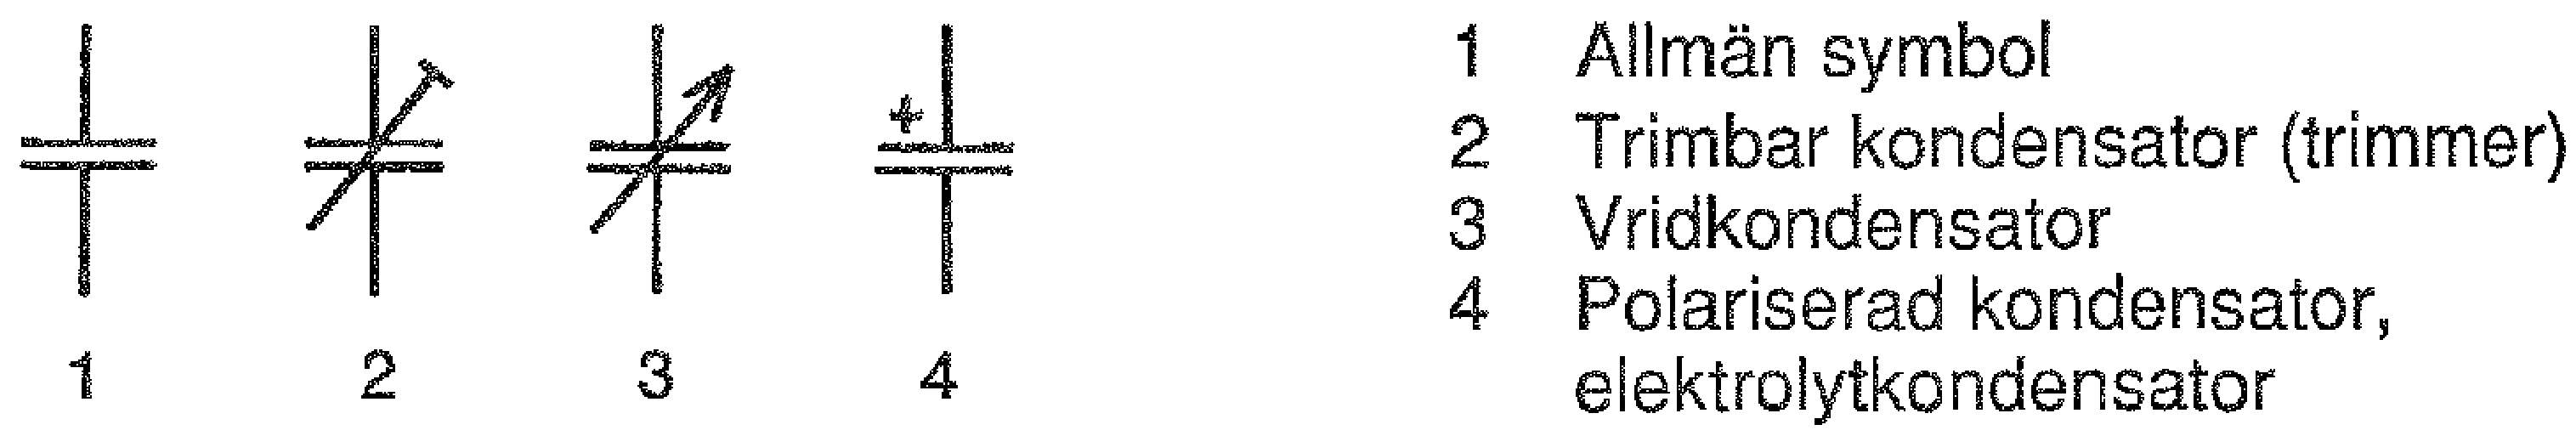
\includegraphics[width=\textwidth]{images/cropped_pdfs/bild_2_2-02.pdf}
\caption{Schemasymboler för kondensatorer}
\label{fig:BildII2-2}
\end{figure}

Bild \ref{fig:BildII2-2}

Kondensatorer har oftast namn efter utförande och det dielektriska materialet.

\emph{Pappers- och plastkondensatorer}

Plattorna i dessa typer består av aluminiumremsor med anslutningstrådar.
Däremellan finns en pappers- respektive plastremsa som dielektrikum. För att
spara plats rullas det hela ihop och skyddas med en plastingjutning.

\emph{Keramiska kondensatorer}

I keramiska kondensatorer består dielektrikum av något keramiskt material.
På ömse sidor om detta sätts en metallbeläggning med anslutningstrådar.

\emph{Glimmerkondensatorer}

I denna kondensatortyp består dielektrikum av tunna glimmerskivor.

\emph{Elektrolytkondensatorer}

Elektrolytkondensatorer har elektroder av aluminium eller tantal där pluspolen
(anoden) ges ett mycket tunt oxidskikt. Detta är inte ledande och fungerar som
dielektrikum. Mellan oxidskiktet och minuspolen (katoden) läggs en elektrolyt
med låg resistivitet.

Elekrolytkondensatorer har särskilt högt kapacitansvärde. Till skillnad från
andra kondensatortyper är elektolytkondensatorer polariserade. Utom i ett
specialfall innebär det att polariteten på den pålagda spänningen inte får
kastas om. Flera olika slags elektrolytkondensatorer finns, bland andra våta
och torra aluminiumelektrolytkondensatorer samt tantalelektrolytkondensatorer.

\subsubsection{Variabla kondensatorer}
Variabla kondensatorer har oftast sitt namn efter utförandeformen, som
vridkondensator och trimbar kondensator (trimmer).

\subsection{Temperaturkoefficient}

På liknande sätt som med resistorer påverkas kapacitansen i kondensatorer av
temperaturen. Att sambandet mellan kapacitans och temperatur är viktigt förstås
av att temperaturkoefficienten i den frekvensbestämmande kapacitansen i en
oscillatorkrets är en av faktorerna för stabil frekvens.

Temperaturkoefficienten \(\alpha _c\) anger kapacitansändringen per grad temperaturändring.
Kapacitansändringen blir då

\[  \Delta C = \pm \alpha _c \cdot C_k \cdot \Delta\vartheta  \]

varvid \(C_k\) är kapacitansvärdet vid den lägre temperaturen (oftast 20~\degree C) och
\(\Delta\vartheta\) är temperaturändringen i kelvin.
Kelvin [K] är den normerade måttenheten för absolut temperatur.
En ändring med 1\,K motsvarar en ändring med 1\degree\,C.

Är \(\alpha _c\) positivt betyder det att kapaciteten ökar med ökande
temperatur. Är \(\alpha _c\) negativt betyder det att kapaciteten minskar med ökande
temperatur.

En kondensator som är märkt med N 100 betyder:
\[ \alpha _c = -100 \cdot 10^{-6} 1/\unit{K}  \]

%\subsection{Standardiserade komponentvärden}
\index{kondensator!standardiserade värden}

Kondensatorer tillverkas vanligen med standardiserade värden från en talserie.

\subsection{Märkning av kondensatorer}

Kondensatorer märks med hjälp av siffror och bokstäver eller med en
färgkod så att kondensatorns huvuddata kan avläsas.
Ofta finns märkningen förklarad i komponentleverantörernas kataloger.
